% Source-faithful topology only; oblique projection is schematic, not a metric drawing.
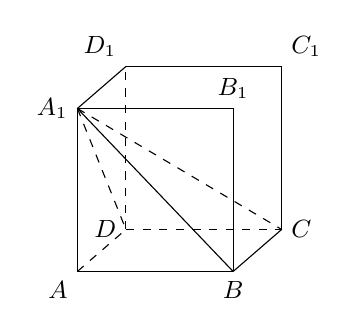
\begin{tikzpicture}[scale=0.92, every node/.style={font=\small}]
  \coordinate (A)  at (0,0);
  \coordinate (B)  at (2.15,0);
  \coordinate (C)  at (2.82,0.58);
  \coordinate (D)  at (0.67,0.58);
  \coordinate (A1) at (0,2.25);
  \coordinate (B1) at (2.15,2.25);
  \coordinate (C1) at (2.82,2.83);
  \coordinate (D1) at (0.67,2.83);

  % Visible prism edges.
  \draw (A) -- (B);
  \draw (B) -- (C);
  \draw (C) -- (C1);
  \draw (C1) -- (D1);
  \draw (D1) -- (A1);
  \draw (A1) -- (B1);
  \draw (B1) -- (B);
  \draw (A) -- (A1);

  % Hidden prism edges.
  \draw[dashed] (A) -- (D);
  \draw[dashed] (D) -- (C);
  \draw[dashed] (D) -- (D1);

  % Auxiliary segments shown in the source diagram.
  \draw (A1) -- (B);
  \draw[dashed] (A1) -- (C);
  \draw[dashed] (A1) -- (D);

  \node[below left] at (A) {$A$};
  \node[below] at (B) {$B$};
  \node[right] at (C) {$C$};
  \node[left] at (D) {$D$};
  \node[left] at (A1) {$A_1$};
  \node[above] at (B1) {$B_1$};
  \node[above right] at (C1) {$C_1$};
  \node[above left] at (D1) {$D_1$};
\end{tikzpicture}
